\section{Introduction}
The emergence of low power wireless systems in past decades was followed closely by attempts at optimizing energy efficiency and power consumption to facilitate long lifetime sensing deployments.  Research in this area was marked by many successes in the form of efficient time synchronization algorithms \r{cite?}, routing protocols \r{cite CTP?}, new sensing paradigms \r{cite CS?}, and the emergence of several widely-adopted operating systems for embedded systems (e.g., \cite{tinyos, contiki}). Newer IC fabrication technologies have introduced several additional variables into the energy management game; in addition to power variation across temperature, power variation on a per-instance level has become a non-trivial factor \cite{borkar2003, gupta2003}. Figure \ref{fig:variation} offers more intuition into the matter, showing the projected variation in idle and overall power as projected by IRTS for years to come \r{cite here} as well as recent variability results in the literature. 

Considerable research has focused on exposing energy and power measurements or estimates to the developer and even to the end user.  For example, techniques using linear combinations of instruction and performance counters \cite{sun2012,singh2009}, activity monitoring strategies \cite{appscope}, and various battery discharge-based models \cite{zhang2010} have been explored as tools for providing system-wide, application-specific, and even per-process granularities of energy usage.  Improved techniques for accurately  estimating and measuring power consumption will enable online power management in ways that were infeasible before, helping mitigate fabrication-induced per-instance chip variation as well \r{cite here?}. 

\begin{figure}
\centering
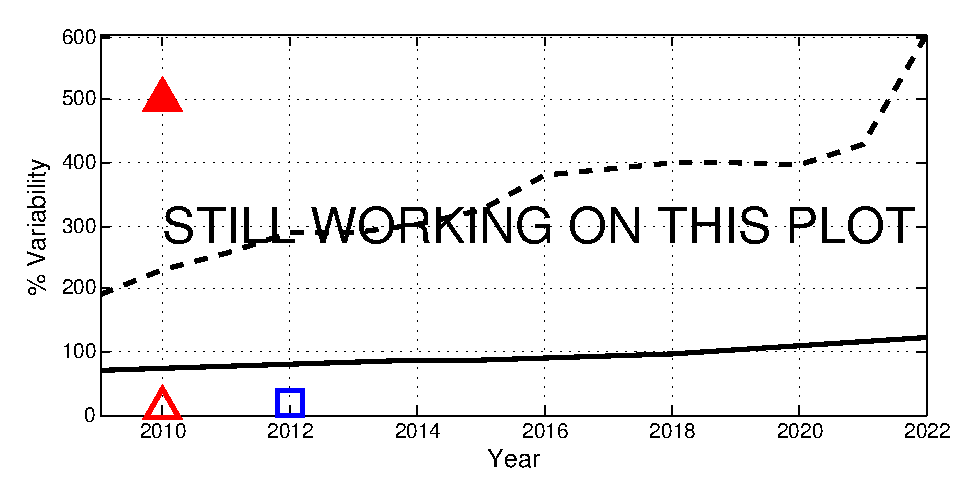
\includegraphics[width=1\columnwidth]{figures/projected_variations.eps}
\caption{\label{fig:variation}IRTS projections for sleep and idle power variability with measurements from recent literature.}
\end{figure}

Perhaps the most widely used and most effective strategies for extending the lifetime of energy-constrained systems are those based on controlling the ratio of active to idle time that the system is allowed, or \emph{duty cycling} a system.  Duty cycled systems take advantage of the disparity between active and idle power consumption, greatly increasing the lifetime of systems where latency and throughput constraints can be relaxed. Because of temperature and instance dependencies in power consumption, however, arriving at an optimal system-wide duty cycle ratio to achieve a lifetime goal given an energy constraint is difficult to do without emph{a priori} knowledge of instance-specific power models and temperature statistics for the target deployment location \cite{wanner2010}. Furthermore, applications involving more than one task introduce notions of fairness and utility---specifically, how should active processor time be distributed between each task so as to maximize the utility of the application and still meet the desired lifetime goal?

In this paper we explore the interplay between variable active and idle power consumption, deployment-specific temperature profiles, and multiple heterogeneous tasks with corresponding duty cycles. Specifically, we seek an answer to the question posed above; in an environment where power and temperature are measurable quantities, we seek an optimal strategy for distributing active processing time between arbitrary tasks so as to maximize application utility.  

Our contributions include the following: (1) we demonstrate an efficient and simple method for online-learning of idle and active power curves which are, in general, nonlinear functions of temperature; (2) we distill the minimum statistics regarding temperature required for accurate system lifetime predictions; (3) we evaluate VaRTOS, a series of kernel extensions to the FreeRTOS operating system that provides explicit treatment and online optimization of multiple-task duty cycles with corresponding utilities; and (4) we evaluate the effects of VaRTOS on several prototypical applications, using a modified version of the QEMU simulation suite \r{cite QEMU}.   



